% Created by tikzDevice version 0.10.1 on 2018-01-23 20:20:44
% !TEX encoding = UTF-8 Unicode
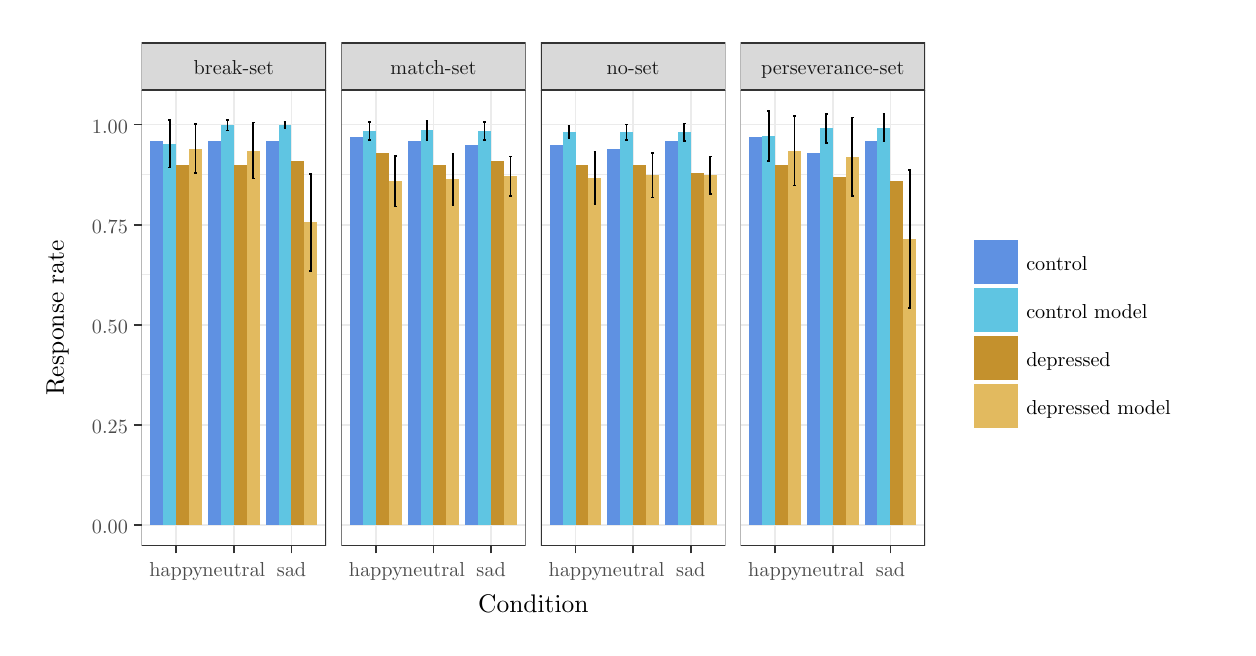
\begin{tikzpicture}[x=1pt,y=1pt]
\definecolor{fillColor}{RGB}{255,255,255}
\path[use as bounding box,fill=fillColor,fill opacity=0.00] (0,0) rectangle (433.62,216.81);
\begin{scope}
\path[clip] (  0.00,  0.00) rectangle (433.62,216.81);
\definecolor{drawColor}{RGB}{255,255,255}
\definecolor{fillColor}{RGB}{255,255,255}

\path[draw=drawColor,line width= 0.6pt,line join=round,line cap=round,fill=fillColor] (  0.00,  0.00) rectangle (433.62,216.81);
\end{scope}
\begin{scope}
\path[clip] ( 41.17, 29.59) rectangle (107.82,194.25);
\definecolor{fillColor}{RGB}{255,255,255}

\path[fill=fillColor] ( 41.17, 29.59) rectangle (107.82,194.25);
\definecolor{drawColor}{gray}{0.92}

\path[draw=drawColor,line width= 0.3pt,line join=round] ( 41.17, 55.16) --
	(107.82, 55.16);

\path[draw=drawColor,line width= 0.3pt,line join=round] ( 41.17, 91.34) --
	(107.82, 91.34);

\path[draw=drawColor,line width= 0.3pt,line join=round] ( 41.17,127.52) --
	(107.82,127.52);

\path[draw=drawColor,line width= 0.3pt,line join=round] ( 41.17,163.69) --
	(107.82,163.69);

\path[draw=drawColor,line width= 0.6pt,line join=round] ( 41.17, 37.07) --
	(107.82, 37.07);

\path[draw=drawColor,line width= 0.6pt,line join=round] ( 41.17, 73.25) --
	(107.82, 73.25);

\path[draw=drawColor,line width= 0.6pt,line join=round] ( 41.17,109.43) --
	(107.82,109.43);

\path[draw=drawColor,line width= 0.6pt,line join=round] ( 41.17,145.61) --
	(107.82,145.61);

\path[draw=drawColor,line width= 0.6pt,line join=round] ( 41.17,181.78) --
	(107.82,181.78);

\path[draw=drawColor,line width= 0.6pt,line join=round] ( 53.67, 29.59) --
	( 53.67,194.25);

\path[draw=drawColor,line width= 0.6pt,line join=round] ( 74.50, 29.59) --
	( 74.50,194.25);

\path[draw=drawColor,line width= 0.6pt,line join=round] ( 95.32, 29.59) --
	( 95.32,194.25);
\definecolor{fillColor}{RGB}{226,186,95}

\path[fill=fillColor] ( 58.36, 37.07) rectangle ( 63.04,173.09);
\definecolor{fillColor}{RGB}{196,145,45}

\path[fill=fillColor] ( 53.67, 37.07) rectangle ( 58.36,167.31);
\definecolor{fillColor}{RGB}{95,197,226}

\path[fill=fillColor] ( 48.98, 37.07) rectangle ( 53.67,174.83);
\definecolor{fillColor}{RGB}{95,145,226}

\path[fill=fillColor] ( 44.30, 37.07) rectangle ( 48.98,176.00);
\definecolor{fillColor}{RGB}{226,186,95}

\path[fill=fillColor] ( 79.18, 37.07) rectangle ( 83.87,172.40);
\definecolor{fillColor}{RGB}{196,145,45}

\path[fill=fillColor] ( 74.50, 37.07) rectangle ( 79.18,167.31);
\definecolor{fillColor}{RGB}{95,197,226}

\path[fill=fillColor] ( 69.81, 37.07) rectangle ( 74.50,181.52);
\definecolor{fillColor}{RGB}{95,145,226}

\path[fill=fillColor] ( 65.12, 37.07) rectangle ( 69.81,176.00);
\definecolor{fillColor}{RGB}{226,186,95}

\path[fill=fillColor] (100.01, 37.07) rectangle (104.69,146.44);
\definecolor{fillColor}{RGB}{196,145,45}

\path[fill=fillColor] ( 95.32, 37.07) rectangle (100.01,168.76);
\definecolor{fillColor}{RGB}{95,197,226}

\path[fill=fillColor] ( 90.64, 37.07) rectangle ( 95.32,181.63);
\definecolor{fillColor}{RGB}{95,145,226}

\path[fill=fillColor] ( 85.95, 37.07) rectangle ( 90.64,176.00);
\definecolor{drawColor}{RGB}{0,0,0}

\path[draw=drawColor,line width= 0.6pt,line join=round] ( 60.18,182.00) --
	( 61.22,182.00);

\path[draw=drawColor,line width= 0.6pt,line join=round] ( 60.70,182.00) --
	( 60.70,164.19);

\path[draw=drawColor,line width= 0.6pt,line join=round] ( 60.18,164.19) --
	( 61.22,164.19);

\path[draw=drawColor,line width= 0.6pt,line join=round] ( 50.81,183.33) --
	( 51.85,183.33);

\path[draw=drawColor,line width= 0.6pt,line join=round] ( 51.33,183.33) --
	( 51.33,166.33);

\path[draw=drawColor,line width= 0.6pt,line join=round] ( 50.81,166.33) --
	( 51.85,166.33);

\path[draw=drawColor,line width= 0.6pt,line join=round] ( 81.00,182.54) --
	( 82.05,182.54);

\path[draw=drawColor,line width= 0.6pt,line join=round] ( 81.52,182.54) --
	( 81.52,162.27);

\path[draw=drawColor,line width= 0.6pt,line join=round] ( 81.00,162.27) --
	( 82.05,162.27);

\path[draw=drawColor,line width= 0.6pt,line join=round] ( 71.63,183.38) --
	( 72.67,183.38);

\path[draw=drawColor,line width= 0.6pt,line join=round] ( 72.15,183.38) --
	( 72.15,179.66);

\path[draw=drawColor,line width= 0.6pt,line join=round] ( 71.63,179.66) --
	( 72.67,179.66);

\path[draw=drawColor,line width= 0.6pt,line join=round] (101.83,164.00) --
	(102.87,164.00);

\path[draw=drawColor,line width= 0.6pt,line join=round] (102.35,164.00) --
	(102.35,128.89);

\path[draw=drawColor,line width= 0.6pt,line join=round] (101.83,128.89) --
	(102.87,128.89);

\path[draw=drawColor,line width= 0.6pt,line join=round] ( 92.46,182.71) --
	( 93.50,182.71);

\path[draw=drawColor,line width= 0.6pt,line join=round] ( 92.98,182.71) --
	( 92.98,180.55);

\path[draw=drawColor,line width= 0.6pt,line join=round] ( 92.46,180.55) --
	( 93.50,180.55);
\definecolor{drawColor}{gray}{0.20}

\path[draw=drawColor,line width= 0.6pt,line join=round,line cap=round] ( 41.17, 29.59) rectangle (107.82,194.25);
\end{scope}
\begin{scope}
\path[clip] (113.32, 29.59) rectangle (179.96,194.25);
\definecolor{fillColor}{RGB}{255,255,255}

\path[fill=fillColor] (113.32, 29.59) rectangle (179.96,194.25);
\definecolor{drawColor}{gray}{0.92}

\path[draw=drawColor,line width= 0.3pt,line join=round] (113.32, 55.16) --
	(179.96, 55.16);

\path[draw=drawColor,line width= 0.3pt,line join=round] (113.32, 91.34) --
	(179.96, 91.34);

\path[draw=drawColor,line width= 0.3pt,line join=round] (113.32,127.52) --
	(179.96,127.52);

\path[draw=drawColor,line width= 0.3pt,line join=round] (113.32,163.69) --
	(179.96,163.69);

\path[draw=drawColor,line width= 0.6pt,line join=round] (113.32, 37.07) --
	(179.96, 37.07);

\path[draw=drawColor,line width= 0.6pt,line join=round] (113.32, 73.25) --
	(179.96, 73.25);

\path[draw=drawColor,line width= 0.6pt,line join=round] (113.32,109.43) --
	(179.96,109.43);

\path[draw=drawColor,line width= 0.6pt,line join=round] (113.32,145.61) --
	(179.96,145.61);

\path[draw=drawColor,line width= 0.6pt,line join=round] (113.32,181.78) --
	(179.96,181.78);

\path[draw=drawColor,line width= 0.6pt,line join=round] (125.81, 29.59) --
	(125.81,194.25);

\path[draw=drawColor,line width= 0.6pt,line join=round] (146.64, 29.59) --
	(146.64,194.25);

\path[draw=drawColor,line width= 0.6pt,line join=round] (167.47, 29.59) --
	(167.47,194.25);
\definecolor{fillColor}{RGB}{226,186,95}

\path[fill=fillColor] (130.50, 37.07) rectangle (135.19,161.29);
\definecolor{fillColor}{RGB}{196,145,45}

\path[fill=fillColor] (125.81, 37.07) rectangle (130.50,171.65);
\definecolor{fillColor}{RGB}{95,197,226}

\path[fill=fillColor] (121.13, 37.07) rectangle (125.81,179.42);
\definecolor{fillColor}{RGB}{95,145,226}

\path[fill=fillColor] (116.44, 37.07) rectangle (121.13,177.44);
\definecolor{fillColor}{RGB}{226,186,95}

\path[fill=fillColor] (151.33, 37.07) rectangle (156.01,162.07);
\definecolor{fillColor}{RGB}{196,145,45}

\path[fill=fillColor] (146.64, 37.07) rectangle (151.33,167.31);
\definecolor{fillColor}{RGB}{95,197,226}

\path[fill=fillColor] (141.95, 37.07) rectangle (146.64,179.69);
\definecolor{fillColor}{RGB}{95,145,226}

\path[fill=fillColor] (137.27, 37.07) rectangle (141.95,176.00);
\definecolor{fillColor}{RGB}{226,186,95}

\path[fill=fillColor] (172.15, 37.07) rectangle (176.84,163.04);
\definecolor{fillColor}{RGB}{196,145,45}

\path[fill=fillColor] (167.47, 37.07) rectangle (172.15,168.76);
\definecolor{fillColor}{RGB}{95,197,226}

\path[fill=fillColor] (162.78, 37.07) rectangle (167.47,179.41);
\definecolor{fillColor}{RGB}{95,145,226}

\path[fill=fillColor] (158.10, 37.07) rectangle (162.78,174.55);
\definecolor{drawColor}{RGB}{0,0,0}

\path[draw=drawColor,line width= 0.6pt,line join=round] (132.32,170.36) --
	(133.36,170.36);

\path[draw=drawColor,line width= 0.6pt,line join=round] (132.84,170.36) --
	(132.84,152.21);

\path[draw=drawColor,line width= 0.6pt,line join=round] (132.32,152.21) --
	(133.36,152.21);

\path[draw=drawColor,line width= 0.6pt,line join=round] (122.95,182.66) --
	(123.99,182.66);

\path[draw=drawColor,line width= 0.6pt,line join=round] (123.47,182.66) --
	(123.47,176.19);

\path[draw=drawColor,line width= 0.6pt,line join=round] (122.95,176.19) --
	(123.99,176.19);

\path[draw=drawColor,line width= 0.6pt,line join=round] (153.15,171.36) --
	(154.19,171.36);

\path[draw=drawColor,line width= 0.6pt,line join=round] (153.67,171.36) --
	(153.67,152.77);

\path[draw=drawColor,line width= 0.6pt,line join=round] (153.15,152.77) --
	(154.19,152.77);

\path[draw=drawColor,line width= 0.6pt,line join=round] (143.78,183.21) --
	(144.82,183.21);

\path[draw=drawColor,line width= 0.6pt,line join=round] (144.30,183.21) --
	(144.30,176.17);

\path[draw=drawColor,line width= 0.6pt,line join=round] (143.78,176.17) --
	(144.82,176.17);

\path[draw=drawColor,line width= 0.6pt,line join=round] (173.98,170.20) --
	(175.02,170.20);

\path[draw=drawColor,line width= 0.6pt,line join=round] (174.50,170.20) --
	(174.50,155.89);

\path[draw=drawColor,line width= 0.6pt,line join=round] (173.98,155.89) --
	(175.02,155.89);

\path[draw=drawColor,line width= 0.6pt,line join=round] (164.60,182.67) --
	(165.64,182.67);

\path[draw=drawColor,line width= 0.6pt,line join=round] (165.12,182.67) --
	(165.12,176.15);

\path[draw=drawColor,line width= 0.6pt,line join=round] (164.60,176.15) --
	(165.64,176.15);
\definecolor{drawColor}{gray}{0.20}

\path[draw=drawColor,line width= 0.6pt,line join=round,line cap=round] (113.32, 29.59) rectangle (179.96,194.25);
\end{scope}
\begin{scope}
\path[clip] (185.46, 29.59) rectangle (252.11,194.25);
\definecolor{fillColor}{RGB}{255,255,255}

\path[fill=fillColor] (185.46, 29.59) rectangle (252.11,194.25);
\definecolor{drawColor}{gray}{0.92}

\path[draw=drawColor,line width= 0.3pt,line join=round] (185.46, 55.16) --
	(252.11, 55.16);

\path[draw=drawColor,line width= 0.3pt,line join=round] (185.46, 91.34) --
	(252.11, 91.34);

\path[draw=drawColor,line width= 0.3pt,line join=round] (185.46,127.52) --
	(252.11,127.52);

\path[draw=drawColor,line width= 0.3pt,line join=round] (185.46,163.69) --
	(252.11,163.69);

\path[draw=drawColor,line width= 0.6pt,line join=round] (185.46, 37.07) --
	(252.11, 37.07);

\path[draw=drawColor,line width= 0.6pt,line join=round] (185.46, 73.25) --
	(252.11, 73.25);

\path[draw=drawColor,line width= 0.6pt,line join=round] (185.46,109.43) --
	(252.11,109.43);

\path[draw=drawColor,line width= 0.6pt,line join=round] (185.46,145.61) --
	(252.11,145.61);

\path[draw=drawColor,line width= 0.6pt,line join=round] (185.46,181.78) --
	(252.11,181.78);

\path[draw=drawColor,line width= 0.6pt,line join=round] (197.96, 29.59) --
	(197.96,194.25);

\path[draw=drawColor,line width= 0.6pt,line join=round] (218.79, 29.59) --
	(218.79,194.25);

\path[draw=drawColor,line width= 0.6pt,line join=round] (239.61, 29.59) --
	(239.61,194.25);
\definecolor{fillColor}{RGB}{226,186,95}

\path[fill=fillColor] (202.64, 37.07) rectangle (207.33,162.66);
\definecolor{fillColor}{RGB}{196,145,45}

\path[fill=fillColor] (197.96, 37.07) rectangle (202.64,167.31);
\definecolor{fillColor}{RGB}{95,197,226}

\path[fill=fillColor] (193.27, 37.07) rectangle (197.96,179.14);
\definecolor{fillColor}{RGB}{95,145,226}

\path[fill=fillColor] (188.59, 37.07) rectangle (193.27,174.55);
\definecolor{fillColor}{RGB}{226,186,95}

\path[fill=fillColor] (223.47, 37.07) rectangle (228.16,163.53);
\definecolor{fillColor}{RGB}{196,145,45}

\path[fill=fillColor] (218.79, 37.07) rectangle (223.47,167.31);
\definecolor{fillColor}{RGB}{95,197,226}

\path[fill=fillColor] (214.10, 37.07) rectangle (218.79,178.99);
\definecolor{fillColor}{RGB}{95,145,226}

\path[fill=fillColor] (209.41, 37.07) rectangle (214.10,173.10);
\definecolor{fillColor}{RGB}{226,186,95}

\path[fill=fillColor] (244.30, 37.07) rectangle (248.98,163.42);
\definecolor{fillColor}{RGB}{196,145,45}

\path[fill=fillColor] (239.61, 37.07) rectangle (244.30,164.42);
\definecolor{fillColor}{RGB}{95,197,226}

\path[fill=fillColor] (234.93, 37.07) rectangle (239.61,179.03);
\definecolor{fillColor}{RGB}{95,145,226}

\path[fill=fillColor] (230.24, 37.07) rectangle (234.93,176.00);
\definecolor{drawColor}{RGB}{0,0,0}

\path[draw=drawColor,line width= 0.6pt,line join=round] (204.47,172.12) --
	(205.51,172.12);

\path[draw=drawColor,line width= 0.6pt,line join=round] (204.99,172.12) --
	(204.99,153.20);

\path[draw=drawColor,line width= 0.6pt,line join=round] (204.47,153.20) --
	(205.51,153.20);

\path[draw=drawColor,line width= 0.6pt,line join=round] (195.10,181.45) --
	(196.14,181.45);

\path[draw=drawColor,line width= 0.6pt,line join=round] (195.62,181.45) --
	(195.62,176.83);

\path[draw=drawColor,line width= 0.6pt,line join=round] (195.10,176.83) --
	(196.14,176.83);

\path[draw=drawColor,line width= 0.6pt,line join=round] (225.29,171.57) --
	(226.34,171.57);

\path[draw=drawColor,line width= 0.6pt,line join=round] (225.81,171.57) --
	(225.81,155.50);

\path[draw=drawColor,line width= 0.6pt,line join=round] (225.29,155.50) --
	(226.34,155.50);

\path[draw=drawColor,line width= 0.6pt,line join=round] (215.92,181.78) --
	(216.96,181.78);

\path[draw=drawColor,line width= 0.6pt,line join=round] (216.44,181.78) --
	(216.44,176.20);

\path[draw=drawColor,line width= 0.6pt,line join=round] (215.92,176.20) --
	(216.96,176.20);

\path[draw=drawColor,line width= 0.6pt,line join=round] (246.12,170.20) --
	(247.16,170.20);

\path[draw=drawColor,line width= 0.6pt,line join=round] (246.64,170.20) --
	(246.64,156.64);

\path[draw=drawColor,line width= 0.6pt,line join=round] (246.12,156.64) --
	(247.16,156.64);

\path[draw=drawColor,line width= 0.6pt,line join=round] (236.75,182.16) --
	(237.79,182.16);

\path[draw=drawColor,line width= 0.6pt,line join=round] (237.27,182.16) --
	(237.27,175.89);

\path[draw=drawColor,line width= 0.6pt,line join=round] (236.75,175.89) --
	(237.79,175.89);
\definecolor{drawColor}{gray}{0.20}

\path[draw=drawColor,line width= 0.6pt,line join=round,line cap=round] (185.46, 29.59) rectangle (252.11,194.25);
\end{scope}
\begin{scope}
\path[clip] (257.61, 29.59) rectangle (324.25,194.25);
\definecolor{fillColor}{RGB}{255,255,255}

\path[fill=fillColor] (257.61, 29.59) rectangle (324.25,194.25);
\definecolor{drawColor}{gray}{0.92}

\path[draw=drawColor,line width= 0.3pt,line join=round] (257.61, 55.16) --
	(324.25, 55.16);

\path[draw=drawColor,line width= 0.3pt,line join=round] (257.61, 91.34) --
	(324.25, 91.34);

\path[draw=drawColor,line width= 0.3pt,line join=round] (257.61,127.52) --
	(324.25,127.52);

\path[draw=drawColor,line width= 0.3pt,line join=round] (257.61,163.69) --
	(324.25,163.69);

\path[draw=drawColor,line width= 0.6pt,line join=round] (257.61, 37.07) --
	(324.25, 37.07);

\path[draw=drawColor,line width= 0.6pt,line join=round] (257.61, 73.25) --
	(324.25, 73.25);

\path[draw=drawColor,line width= 0.6pt,line join=round] (257.61,109.43) --
	(324.25,109.43);

\path[draw=drawColor,line width= 0.6pt,line join=round] (257.61,145.61) --
	(324.25,145.61);

\path[draw=drawColor,line width= 0.6pt,line join=round] (257.61,181.78) --
	(324.25,181.78);

\path[draw=drawColor,line width= 0.6pt,line join=round] (270.10, 29.59) --
	(270.10,194.25);

\path[draw=drawColor,line width= 0.6pt,line join=round] (290.93, 29.59) --
	(290.93,194.25);

\path[draw=drawColor,line width= 0.6pt,line join=round] (311.76, 29.59) --
	(311.76,194.25);
\definecolor{fillColor}{RGB}{226,186,95}

\path[fill=fillColor] (274.79, 37.07) rectangle (279.48,172.29);
\definecolor{fillColor}{RGB}{196,145,45}

\path[fill=fillColor] (270.10, 37.07) rectangle (274.79,167.31);
\definecolor{fillColor}{RGB}{95,197,226}

\path[fill=fillColor] (265.42, 37.07) rectangle (270.10,177.66);
\definecolor{fillColor}{RGB}{95,145,226}

\path[fill=fillColor] (260.73, 37.07) rectangle (265.42,177.44);
\definecolor{fillColor}{RGB}{226,186,95}

\path[fill=fillColor] (295.62, 37.07) rectangle (300.30,170.15);
\definecolor{fillColor}{RGB}{196,145,45}

\path[fill=fillColor] (290.93, 37.07) rectangle (295.62,162.97);
\definecolor{fillColor}{RGB}{95,197,226}

\path[fill=fillColor] (286.24, 37.07) rectangle (290.93,180.39);
\definecolor{fillColor}{RGB}{95,145,226}

\path[fill=fillColor] (281.56, 37.07) rectangle (286.24,171.65);
\definecolor{fillColor}{RGB}{226,186,95}

\path[fill=fillColor] (316.44, 37.07) rectangle (321.13,140.39);
\definecolor{fillColor}{RGB}{196,145,45}

\path[fill=fillColor] (311.76, 37.07) rectangle (316.44,161.52);
\definecolor{fillColor}{RGB}{95,197,226}

\path[fill=fillColor] (307.07, 37.07) rectangle (311.76,180.57);
\definecolor{fillColor}{RGB}{95,145,226}

\path[fill=fillColor] (302.39, 37.07) rectangle (307.07,176.00);
\definecolor{drawColor}{RGB}{0,0,0}

\path[draw=drawColor,line width= 0.6pt,line join=round] (276.61,184.78) --
	(277.65,184.78);

\path[draw=drawColor,line width= 0.6pt,line join=round] (277.13,184.78) --
	(277.13,159.81);

\path[draw=drawColor,line width= 0.6pt,line join=round] (276.61,159.81) --
	(277.65,159.81);

\path[draw=drawColor,line width= 0.6pt,line join=round] (267.24,186.76) --
	(268.28,186.76);

\path[draw=drawColor,line width= 0.6pt,line join=round] (267.76,186.76) --
	(267.76,168.56);

\path[draw=drawColor,line width= 0.6pt,line join=round] (267.24,168.56) --
	(268.28,168.56);

\path[draw=drawColor,line width= 0.6pt,line join=round] (297.44,184.38) --
	(298.48,184.38);

\path[draw=drawColor,line width= 0.6pt,line join=round] (297.96,184.38) --
	(297.96,155.91);

\path[draw=drawColor,line width= 0.6pt,line join=round] (297.44,155.91) --
	(298.48,155.91);

\path[draw=drawColor,line width= 0.6pt,line join=round] (288.07,185.54) --
	(289.11,185.54);

\path[draw=drawColor,line width= 0.6pt,line join=round] (288.59,185.54) --
	(288.59,175.23);

\path[draw=drawColor,line width= 0.6pt,line join=round] (288.07,175.23) --
	(289.11,175.23);

\path[draw=drawColor,line width= 0.6pt,line join=round] (318.27,165.32) --
	(319.31,165.32);

\path[draw=drawColor,line width= 0.6pt,line join=round] (318.79,165.32) --
	(318.79,115.46);

\path[draw=drawColor,line width= 0.6pt,line join=round] (318.27,115.46) --
	(319.31,115.46);

\path[draw=drawColor,line width= 0.6pt,line join=round] (308.89,185.50) --
	(309.93,185.50);

\path[draw=drawColor,line width= 0.6pt,line join=round] (309.41,185.50) --
	(309.41,175.63);

\path[draw=drawColor,line width= 0.6pt,line join=round] (308.89,175.63) --
	(309.93,175.63);
\definecolor{drawColor}{gray}{0.20}

\path[draw=drawColor,line width= 0.6pt,line join=round,line cap=round] (257.61, 29.59) rectangle (324.25,194.25);
\end{scope}
\begin{scope}
\path[clip] ( 41.17,194.25) rectangle (107.82,211.31);
\definecolor{drawColor}{gray}{0.20}
\definecolor{fillColor}{gray}{0.85}

\path[draw=drawColor,line width= 0.6pt,line join=round,line cap=round,fill=fillColor] ( 41.17,194.25) rectangle (107.82,211.31);
\definecolor{drawColor}{gray}{0.10}

\node[text=drawColor,anchor=base,inner sep=0pt, outer sep=0pt, scale=  0.73] at ( 74.50,199.75) {break-set};
\end{scope}
\begin{scope}
\path[clip] (113.32,194.25) rectangle (179.96,211.31);
\definecolor{drawColor}{gray}{0.20}
\definecolor{fillColor}{gray}{0.85}

\path[draw=drawColor,line width= 0.6pt,line join=round,line cap=round,fill=fillColor] (113.32,194.25) rectangle (179.96,211.31);
\definecolor{drawColor}{gray}{0.10}

\node[text=drawColor,anchor=base,inner sep=0pt, outer sep=0pt, scale=  0.73] at (146.64,199.75) {match-set};
\end{scope}
\begin{scope}
\path[clip] (185.46,194.25) rectangle (252.11,211.31);
\definecolor{drawColor}{gray}{0.20}
\definecolor{fillColor}{gray}{0.85}

\path[draw=drawColor,line width= 0.6pt,line join=round,line cap=round,fill=fillColor] (185.46,194.25) rectangle (252.11,211.31);
\definecolor{drawColor}{gray}{0.10}

\node[text=drawColor,anchor=base,inner sep=0pt, outer sep=0pt, scale=  0.73] at (218.79,199.75) {no-set};
\end{scope}
\begin{scope}
\path[clip] (257.61,194.25) rectangle (324.25,211.31);
\definecolor{drawColor}{gray}{0.20}
\definecolor{fillColor}{gray}{0.85}

\path[draw=drawColor,line width= 0.6pt,line join=round,line cap=round,fill=fillColor] (257.61,194.25) rectangle (324.25,211.31);
\definecolor{drawColor}{gray}{0.10}

\node[text=drawColor,anchor=base,inner sep=0pt, outer sep=0pt, scale=  0.73] at (290.93,199.75) {perseverance-set};
\end{scope}
\begin{scope}
\path[clip] (  0.00,  0.00) rectangle (433.62,216.81);
\definecolor{drawColor}{gray}{0.20}

\path[draw=drawColor,line width= 0.6pt,line join=round] ( 53.67, 26.84) --
	( 53.67, 29.59);

\path[draw=drawColor,line width= 0.6pt,line join=round] ( 74.50, 26.84) --
	( 74.50, 29.59);

\path[draw=drawColor,line width= 0.6pt,line join=round] ( 95.32, 26.84) --
	( 95.32, 29.59);
\end{scope}
\begin{scope}
\path[clip] (  0.00,  0.00) rectangle (433.62,216.81);
\definecolor{drawColor}{gray}{0.30}

\node[text=drawColor,anchor=base,inner sep=0pt, outer sep=0pt, scale=  0.73] at ( 53.67, 18.58) {happy};

\node[text=drawColor,anchor=base,inner sep=0pt, outer sep=0pt, scale=  0.73] at ( 74.50, 18.58) {neutral};

\node[text=drawColor,anchor=base,inner sep=0pt, outer sep=0pt, scale=  0.73] at ( 95.32, 18.58) {sad};
\end{scope}
\begin{scope}
\path[clip] (  0.00,  0.00) rectangle (433.62,216.81);
\definecolor{drawColor}{gray}{0.20}

\path[draw=drawColor,line width= 0.6pt,line join=round] (125.81, 26.84) --
	(125.81, 29.59);

\path[draw=drawColor,line width= 0.6pt,line join=round] (146.64, 26.84) --
	(146.64, 29.59);

\path[draw=drawColor,line width= 0.6pt,line join=round] (167.47, 26.84) --
	(167.47, 29.59);
\end{scope}
\begin{scope}
\path[clip] (  0.00,  0.00) rectangle (433.62,216.81);
\definecolor{drawColor}{gray}{0.30}

\node[text=drawColor,anchor=base,inner sep=0pt, outer sep=0pt, scale=  0.73] at (125.81, 18.58) {happy};

\node[text=drawColor,anchor=base,inner sep=0pt, outer sep=0pt, scale=  0.73] at (146.64, 18.58) {neutral};

\node[text=drawColor,anchor=base,inner sep=0pt, outer sep=0pt, scale=  0.73] at (167.47, 18.58) {sad};
\end{scope}
\begin{scope}
\path[clip] (  0.00,  0.00) rectangle (433.62,216.81);
\definecolor{drawColor}{gray}{0.20}

\path[draw=drawColor,line width= 0.6pt,line join=round] (197.96, 26.84) --
	(197.96, 29.59);

\path[draw=drawColor,line width= 0.6pt,line join=round] (218.79, 26.84) --
	(218.79, 29.59);

\path[draw=drawColor,line width= 0.6pt,line join=round] (239.61, 26.84) --
	(239.61, 29.59);
\end{scope}
\begin{scope}
\path[clip] (  0.00,  0.00) rectangle (433.62,216.81);
\definecolor{drawColor}{gray}{0.30}

\node[text=drawColor,anchor=base,inner sep=0pt, outer sep=0pt, scale=  0.73] at (197.96, 18.58) {happy};

\node[text=drawColor,anchor=base,inner sep=0pt, outer sep=0pt, scale=  0.73] at (218.79, 18.58) {neutral};

\node[text=drawColor,anchor=base,inner sep=0pt, outer sep=0pt, scale=  0.73] at (239.61, 18.58) {sad};
\end{scope}
\begin{scope}
\path[clip] (  0.00,  0.00) rectangle (433.62,216.81);
\definecolor{drawColor}{gray}{0.20}

\path[draw=drawColor,line width= 0.6pt,line join=round] (270.10, 26.84) --
	(270.10, 29.59);

\path[draw=drawColor,line width= 0.6pt,line join=round] (290.93, 26.84) --
	(290.93, 29.59);

\path[draw=drawColor,line width= 0.6pt,line join=round] (311.76, 26.84) --
	(311.76, 29.59);
\end{scope}
\begin{scope}
\path[clip] (  0.00,  0.00) rectangle (433.62,216.81);
\definecolor{drawColor}{gray}{0.30}

\node[text=drawColor,anchor=base,inner sep=0pt, outer sep=0pt, scale=  0.73] at (270.10, 18.58) {happy};

\node[text=drawColor,anchor=base,inner sep=0pt, outer sep=0pt, scale=  0.73] at (290.93, 18.58) {neutral};

\node[text=drawColor,anchor=base,inner sep=0pt, outer sep=0pt, scale=  0.73] at (311.76, 18.58) {sad};
\end{scope}
\begin{scope}
\path[clip] (  0.00,  0.00) rectangle (433.62,216.81);
\definecolor{drawColor}{gray}{0.30}

\node[text=drawColor,anchor=base east,inner sep=0pt, outer sep=0pt, scale=  0.73] at ( 36.22, 34.04) {0.00};

\node[text=drawColor,anchor=base east,inner sep=0pt, outer sep=0pt, scale=  0.73] at ( 36.22, 70.22) {0.25};

\node[text=drawColor,anchor=base east,inner sep=0pt, outer sep=0pt, scale=  0.73] at ( 36.22,106.40) {0.50};

\node[text=drawColor,anchor=base east,inner sep=0pt, outer sep=0pt, scale=  0.73] at ( 36.22,142.58) {0.75};

\node[text=drawColor,anchor=base east,inner sep=0pt, outer sep=0pt, scale=  0.73] at ( 36.22,178.75) {1.00};
\end{scope}
\begin{scope}
\path[clip] (  0.00,  0.00) rectangle (433.62,216.81);
\definecolor{drawColor}{gray}{0.20}

\path[draw=drawColor,line width= 0.6pt,line join=round] ( 38.42, 37.07) --
	( 41.17, 37.07);

\path[draw=drawColor,line width= 0.6pt,line join=round] ( 38.42, 73.25) --
	( 41.17, 73.25);

\path[draw=drawColor,line width= 0.6pt,line join=round] ( 38.42,109.43) --
	( 41.17,109.43);

\path[draw=drawColor,line width= 0.6pt,line join=round] ( 38.42,145.61) --
	( 41.17,145.61);

\path[draw=drawColor,line width= 0.6pt,line join=round] ( 38.42,181.78) --
	( 41.17,181.78);
\end{scope}
\begin{scope}
\path[clip] (  0.00,  0.00) rectangle (433.62,216.81);
\definecolor{drawColor}{RGB}{0,0,0}

\node[text=drawColor,anchor=base,inner sep=0pt, outer sep=0pt, scale=  0.92] at (182.71,  5.50) {Condition};
\end{scope}
\begin{scope}
\path[clip] (  0.00,  0.00) rectangle (433.62,216.81);
\definecolor{drawColor}{RGB}{0,0,0}

\node[text=drawColor,rotate= 90.00,anchor=base,inner sep=0pt, outer sep=0pt, scale=  0.92] at ( 13.08,111.92) {Response rate};
\end{scope}
\begin{scope}
\path[clip] (  0.00,  0.00) rectangle (433.62,216.81);
\definecolor{fillColor}{RGB}{255,255,255}

\path[fill=fillColor] (335.63, 65.58) rectangle (428.12,158.25);
\end{scope}
\begin{scope}
\path[clip] (  0.00,  0.00) rectangle (433.62,216.81);
\definecolor{fillColor}{RGB}{255,255,255}

\path[fill=fillColor] (341.32,123.31) rectangle (358.67,140.65);
\end{scope}
\begin{scope}
\path[clip] (  0.00,  0.00) rectangle (433.62,216.81);
\definecolor{fillColor}{RGB}{95,145,226}

\path[fill=fillColor] (342.04,124.02) rectangle (357.96,139.94);
\end{scope}
\begin{scope}
\path[clip] (  0.00,  0.00) rectangle (433.62,216.81);
\definecolor{fillColor}{RGB}{255,255,255}

\path[fill=fillColor] (341.32,105.96) rectangle (358.67,123.31);
\end{scope}
\begin{scope}
\path[clip] (  0.00,  0.00) rectangle (433.62,216.81);
\definecolor{fillColor}{RGB}{95,197,226}

\path[fill=fillColor] (342.04,106.67) rectangle (357.96,122.60);
\end{scope}
\begin{scope}
\path[clip] (  0.00,  0.00) rectangle (433.62,216.81);
\definecolor{fillColor}{RGB}{255,255,255}

\path[fill=fillColor] (341.32, 88.62) rectangle (358.67,105.96);
\end{scope}
\begin{scope}
\path[clip] (  0.00,  0.00) rectangle (433.62,216.81);
\definecolor{fillColor}{RGB}{196,145,45}

\path[fill=fillColor] (342.04, 89.33) rectangle (357.96,105.25);
\end{scope}
\begin{scope}
\path[clip] (  0.00,  0.00) rectangle (433.62,216.81);
\definecolor{fillColor}{RGB}{255,255,255}

\path[fill=fillColor] (341.32, 71.27) rectangle (358.67, 88.62);
\end{scope}
\begin{scope}
\path[clip] (  0.00,  0.00) rectangle (433.62,216.81);
\definecolor{fillColor}{RGB}{226,186,95}

\path[fill=fillColor] (342.04, 71.98) rectangle (357.96, 87.91);
\end{scope}
\begin{scope}
\path[clip] (  0.00,  0.00) rectangle (433.62,216.81);
\definecolor{drawColor}{RGB}{0,0,0}

\node[text=drawColor,anchor=base west,inner sep=0pt, outer sep=0pt, scale=  0.73] at (360.84,128.95) {control};
\end{scope}
\begin{scope}
\path[clip] (  0.00,  0.00) rectangle (433.62,216.81);
\definecolor{drawColor}{RGB}{0,0,0}

\node[text=drawColor,anchor=base west,inner sep=0pt, outer sep=0pt, scale=  0.73] at (360.84,111.60) {control model};
\end{scope}
\begin{scope}
\path[clip] (  0.00,  0.00) rectangle (433.62,216.81);
\definecolor{drawColor}{RGB}{0,0,0}

\node[text=drawColor,anchor=base west,inner sep=0pt, outer sep=0pt, scale=  0.73] at (360.84, 94.26) {depressed};
\end{scope}
\begin{scope}
\path[clip] (  0.00,  0.00) rectangle (433.62,216.81);
\definecolor{drawColor}{RGB}{0,0,0}

\node[text=drawColor,anchor=base west,inner sep=0pt, outer sep=0pt, scale=  0.73] at (360.84, 76.91) {depressed model};
\end{scope}
\end{tikzpicture}
